\chapter{Microtubule Structure \& Function}
\label{ch:microtubule-structure-function}

\textbf{Microtubules are the ``scaffolding'' of your cells}---tiny hollow tubes made of proteins that give cells their shape and move things around. They're incredibly small: 25 nanometers wide (1/4000th the width of a human hair).

\textbf{What they definitely do:}
\begin{itemize}
\item \textbf{Structural support:} Like steel beams, they keep cells rigid
\item \textbf{Transportation highways:} Roads for ``molecular trucks'' (motor proteins)
\item \textbf{Cell division:} Pull chromosomes apart during cell division
\item \textbf{Movement:} Form the core of sperm tails and lung cilia
\end{itemize}

\textbf{The quantum controversy:} Some scientists propose that microtubules in brain cells might use quantum mechanics to process information or even generate consciousness. This is \emph{highly speculative}---most neuroscientists are skeptical because brains are too warm and wet for quantum effects (which usually need extreme cold and isolation).

\textbf{Current status:} Microtubules are essential for cell function (proven). Whether they do anything quantum-related in the brain remains an open question requiring better experiments.
\section{Overview}

\textbf{Microtubules} are cylindrical protein polymers (25~nm diameter, 15~nm lumen) that form part of the cytoskeleton in eukaryotic cells. They consist of $\alpha$-$\beta$ tubulin heterodimers polymerized into 13 protofilaments arranged in a hollow tube.

\begin{keyconcept}
Microtubules perform \textbf{established biological functions} (structural support, intracellular transport, cell division) with well-understood classical mechanics. The hypothesis that they enable \textbf{quantum information processing in neurons} remains highly speculative and controversial.
\end{keyconcept}

\textbf{Established roles:}
\begin{itemize}
\item Structural support (Young's modulus $\sim$1--2~GPa)
\item Intracellular transport (kinesin and dynein motor tracks)
\item Cell division (mitotic spindle formation)
\item Cilia and flagella (9+2 axoneme motility)
\end{itemize}

\textbf{Speculative quantum roles:}
\begin{itemize}
\item Quantum computation substrates (unproven)
\item Consciousness generation via Orch-OR theory (controversial)
\item Information integration beyond classical neural networks (no experimental evidence)
\end{itemize}

\section{Molecular Structure and Assembly}

\subsection{Tubulin Dimers}

The fundamental building block of microtubules is the $\alpha$-$\beta$ tubulin heterodimer:

\textbf{Composition:}
\begin{itemize}
\item \textbf{$\alpha$-tubulin}: 451 amino acids, $\sim$50~kDa, globular protein
\item \textbf{$\beta$-tubulin}: 445 amino acids, $\sim$50~kDa, globular protein
\item \textbf{Dimer dimensions}: 8~nm long, 4~nm diameter
\item \textbf{GTP binding}: Both subunits have nucleotide-binding sites; $\beta$-tubulin is hydrolysis-active
\end{itemize}

\textbf{Key structural features:}
\begin{itemize}
\item \textbf{Aromatic residues}: 16 Trp, 25 Tyr, 39 Phe per dimer (potential quantum chromophores in speculative theories)
\item \textbf{Hydrophobic core}: Stabilizes folded structure
\item \textbf{C-terminal tail}: Acidic, flexible, extends from surface ($\sim$15 amino acids)
\end{itemize}

The tubulin dimer structure was resolved to 3.5~Å resolution by Nogales et al.~(1998), providing the molecular basis for understanding microtubule assembly.

\subsection{Protofilaments and Lattice Architecture}

\textbf{Assembly hierarchy:}
\begin{enumerate}
\item Tubulin dimers polymerize head-to-tail $\rightarrow$ \textbf{protofilament}
\item 13 protofilaments associate laterally $\rightarrow$ cylindrical microtubule
\end{enumerate}

\textbf{Geometric parameters:}
\begin{equation}
D_{\mathrm{outer}} = 25\ \mathrm{nm}, \quad D_{\mathrm{inner}} = 15\ \mathrm{nm}, \quad t_{\mathrm{wall}} = 5\ \mathrm{nm}
\end{equation}
where:
\begin{itemize}
\item $D_{\mathrm{outer}}$ = outer diameter
\item $D_{\mathrm{inner}}$ = inner (lumen) diameter
\item $t_{\mathrm{wall}}$ = wall thickness
\end{itemize}

\begin{center}
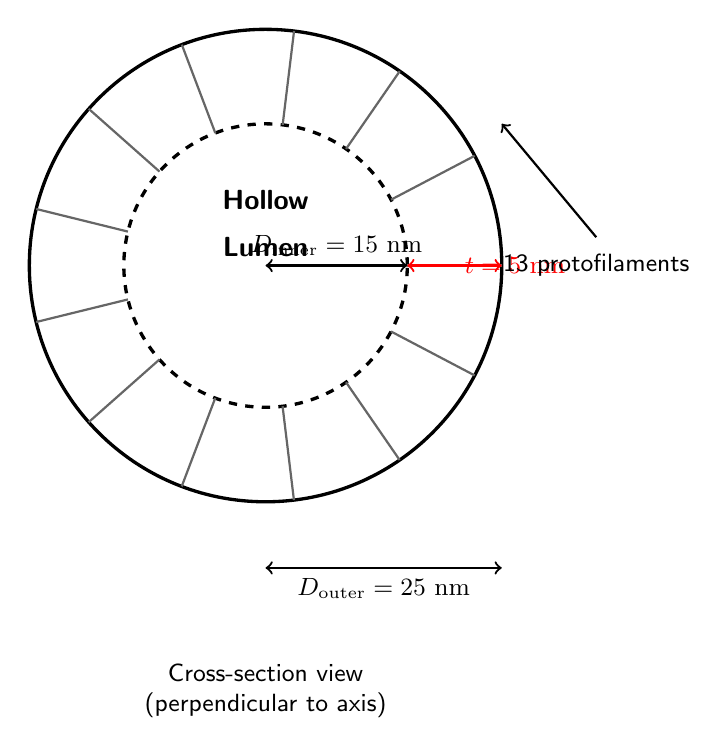
\begin{tikzpicture}[scale=1.2]
% Cross-section view of microtubule
\draw[very thick] (0,0) circle (2.5cm);
\draw[very thick,dashed] (0,0) circle (1.5cm);

% 13 protofilaments (represented as radial segments)
\foreach \angle in {0,27.69,...,360} {
    \draw[thick,black!60] (\angle:1.5cm) -- (\angle:2.5cm);
}

% Dimensions
\draw[<->,thick] (0,0) -- node[above,font=\small] {$D_{\mathrm{inner}}=15$~nm} (1.5,0);
\draw[<->,thick] (0,-3.2) -- node[below,font=\small] {$D_{\mathrm{outer}}=25$~nm} (2.5,-3.2);
\draw[<->,thick,red] (0:1.5) -- node[right,font=\small,red] {$t=5$~nm} (0:2.5);

% Labels
\node[font=\sffamily\bfseries] at (0,0.7) {Hollow};
\node[font=\sffamily\bfseries] at (0,0.2) {Lumen};
\node[font=\sffamily\small] at (3.5,0) {13 protofilaments};
\draw[->,thick] (3.5,0.3) -- (2.5,1.5);

% Tubulin dimers indicator
\node[font=\sffamily\small,align=center] at (0,-4.5) {Cross-section view\\(perpendicular to axis)};
\end{tikzpicture}
\end{center}

\textbf{Helical geometry:}
\begin{itemize}
\item \textbf{Helical pitch}: $h = 12.5$~nm (3-start helix for 13-protofilament structure)
\item \textbf{Lattice seam}: Lateral contacts slightly different at one position (breaks rotational symmetry)
\item \textbf{Polarity}: Plus end ($\beta$-tubulin exposed) vs.~minus end ($\alpha$-tubulin exposed)
\end{itemize}

\textbf{Lattice types:}
\begin{itemize}
\item \textbf{A-lattice}: Straight protofilaments, perfect alignment (most common in vivo)
\item \textbf{B-lattice}: Helical protofilaments, staggered alignment (some in vitro conditions)
\end{itemize}

\subsection{Dynamic Instability}

\textbf{Phenomenon:} Microtubules stochastically switch between growth and rapid shrinkage---a behavior discovered by Mitchison \& Kirschner (1984) that is fundamental to cytoskeletal reorganization.

\textbf{Mechanism:}
\begin{enumerate}
\item \textbf{GTP cap}: Newly added tubulin dimers have GTP bound to $\beta$-tubulin
\item \textbf{Hydrolysis}: GTP $\rightarrow$ GDP after incorporation (delayed by $\tau_{\mathrm{hyd}} \sim 1$~s)
\item \textbf{Catastrophe}: If GTP cap is lost, GDP-tubulin (unstable) is exposed $\rightarrow$ rapid depolymerization
\item \textbf{Rescue}: Occasional stabilization events re-establish growth
\end{enumerate}

\begin{center}
\begin{tikzpicture}[scale=1.0,
  state/.style={rectangle,draw,thick,minimum width=2.5cm,minimum height=1cm,font=\sffamily\small},
  node distance=3.5cm]
  
\node[state] (growth) {GROWTH\\$v_+ \sim 2$ $\mu$m/min};
\node[state,right of=growth] (shrink) {SHRINKAGE\\$v_- \sim 15$ $\mu$m/min};

\draw[->,thick,bend left=30] (growth) to node[above,font=\scriptsize] {Catastrophe ($f_{\mathrm{cat}} \sim 0.01$ s$^{-1}$)} (shrink);
\draw[->,thick,bend left=30] (shrink) to node[below,font=\scriptsize] {Rescue ($f_{\mathrm{res}} \sim 0.001$ s$^{-1}$)} (growth);

% Annotations
\node[below=0.2cm of growth,font=\small,align=center] {GTP cap\\stable};
\node[below=0.2cm of shrink,font=\small,align=center] {GDP exposed\\unstable};

\node[above=1.5cm of growth,xshift=1.5cm,font=\sffamily\small,align=left] {Parameters (in vitro, 37$^\circ$C):};
\end{tikzpicture}
\end{center}

\textbf{Quantitative parameters} (in vitro, 37$^\circ$C):

\begin{equation}
v_+ = 2\ \mu\mathrm{m/min}, \quad v_- = 10\text{--}20\ \mu\mathrm{m/min}
\end{equation}
\begin{equation}
f_{\mathrm{cat}} = 0.01\ \mathrm{s}^{-1}, \quad f_{\mathrm{res}} = 0.001\ \mathrm{s}^{-1}
\end{equation}
where:
\begin{itemize}
\item $v_+$ = growth velocity (plus-end)
\item $v_-$ = shrinkage velocity
\item $f_{\mathrm{cat}}$ = catastrophe frequency
\item $f_{\mathrm{res}}$ = rescue frequency
\end{itemize}

\textbf{Biological function:} Dynamic instability enables rapid cytoskeletal reorganization during mitosis, cell migration, and axon guidance.

\subsection{2. Cellular Functions (Established
)}\label{cellular-functions-established}

\subsubsection{2.1 Structural Support}\label{structural-support}

Microtubules provide mechanical rigidity to cells through their exceptional stiffness:

\textbf{Young's modulus:}
\begin{equation}
E = 1\text{--}2\ \mathrm{GPa}
\end{equation}
where $E$ is Young's modulus (stiffer than actin filaments at $\sim$2~MPa).

\textbf{Persistence length:}
\begin{equation}
L_p = \frac{EI}{k_B T} \approx 5\ \mathrm{mm}
\end{equation}
where:
\begin{itemize}
\item $L_p$ = persistence length (measure of bending stiffness)
\item $I$ = second moment of area (hollow cylinder geometry)
\item $k_B$ = Boltzmann constant ($1.38 \times 10^{-23}$~J/K)
\item $T$ = absolute temperature (K)
\end{itemize}

\textbf{Buckling force:}
\begin{equation}
F_{\mathrm{buckle}} = \frac{\pi^2 EI}{L^2} \approx 5\ \mathrm{pN}
\end{equation}
where $L$ is the length of the microtubule segment.

\begin{calloutbox}{Physical Interpretation}
A persistence length of $L_p \sim 5$~mm is enormous compared to typical cell dimensions (10--100~$\mu$m), meaning microtubules are essentially rigid rods on cellular scales. This rigidity enables them to maintain cell shape and resist compressive loads.
\end{calloutbox}

\subsection{Intracellular Transport}

Microtubules serve as tracks for molecular motor proteins that transport cargo throughout the cell.

\textbf{Motor proteins:}
\begin{itemize}
\item \textbf{Kinesin}: Moves toward plus end (anterograde transport in axons)
\item \textbf{Dynein}: Moves toward minus end (retrograde transport)
\end{itemize}

\textbf{Motor performance:}
\begin{equation}
v_{\mathrm{motor}} \approx 1\ \mu\mathrm{m/s}, \quad F_{\mathrm{motor}} \approx 5\text{--}7\ \mathrm{pN}
\end{equation}
where:
\begin{itemize}
\item $v_{\mathrm{motor}}$ = motor velocity
\item $F_{\mathrm{motor}}$ = stall force (maximum pulling force)
\end{itemize}

\textbf{Cargo:} Vesicles, mitochondria, mRNA granules, protein complexes

\begin{importantbox}
\textbf{Medical relevance:} Defects in axonal transport are linked to neurodegenerative diseases including Alzheimer's disease and amyotrophic lateral sclerosis (ALS). Disrupted cargo transport leads to accumulation of toxic proteins and organelle dysfunction.
\end{importantbox}

\subsection{Mitotic Spindle}

\textbf{Function:} Segregate chromosomes during cell division with high fidelity.

\textbf{Structure:}
\begin{itemize}
\item \textbf{Astral microtubules}: Extend from centrosomes to cell cortex
\item \textbf{Kinetochore microtubules}: Attach to chromosomes
\item \textbf{Interpolar microtubules}: Overlap at spindle midzone
\end{itemize}

\textbf{Force generation:}
\begin{equation}
F_{\mathrm{chrom}} \approx 10\ \mathrm{pN}
\end{equation}
where $F_{\mathrm{chrom}}$ is the force exerted on each chromosome by depolymerizing kinetochore microtubules.

\subsection{Cilia and Flagella}

\textbf{Structure:} \textbf{9+2 axoneme} (9 doublet microtubules + 2 central singlets)

\textbf{Mechanism:} Dynein arms on doublets cause sliding $\rightarrow$ bending motion

\textbf{Beat frequency:}
\begin{equation}
f_{\mathrm{beat}} = 10\text{--}60\ \mathrm{Hz}
\end{equation}
where $f_{\mathrm{beat}}$ depends on cilium/flagellum type and physiological conditions.

\textbf{Examples:}
\begin{itemize}
\item \textbf{Respiratory cilia}: Clear mucus from airways (10--20~Hz)
\item \textbf{Sperm flagella}: Propulsion ($\sim$60~Hz beat frequency)
\item \textbf{Nodal cilia}: Establish left-right asymmetry in embryos
\end{itemize}

\section{Neural Microtubules: Unique Features}

\subsection{Neuronal Cytoskeleton Organization}

\textbf{Axons:}
\begin{itemize}
\item Microtubules uniformly oriented (plus-ends distal)
\item Continuous tracks for kinesin transport
\item Stabilized by tau protein (hyperphosphorylation in Alzheimer's disease)
\end{itemize}

\textbf{Dendrites:}
\begin{itemize}
\item Mixed polarity microtubules
\item Both kinesin and dynein active
\item Dynamic remodeling during synaptic plasticity
\end{itemize}

\textbf{Microtubule density:}
\begin{equation}
N_{\mathrm{MT}} \sim 10^6\ \text{microtubules per neuron}
\end{equation}
where $N_{\mathrm{MT}}$ varies with neuron type and maturation state.

\subsection{Post-Translational Modifications (PTMs)}

\textbf{Tubulin code:} $\sim$20 different PTMs create functional diversity, analogous to the histone code in chromatin.

\textbf{Key modifications:}
\begin{itemize}
\item \textbf{Acetylation} (Lys-40 on $\alpha$-tubulin): Marks stable, long-lived microtubules
\item \textbf{Tyrosination/detyrosination}: Regulates motor protein binding
\item \textbf{Polyglutamylation}: C-terminal tail modification (affects MAP binding)
\item \textbf{Phosphorylation}: Tau phosphorylation regulates microtubule stability
\end{itemize}

\textbf{Function:} PTMs create binding codes for MAPs (microtubule-associated proteins), motors, and signaling proteins, enabling context-dependent regulation of cytoskeletal function.

\subsection{Microtubule-Associated Proteins (MAPs)}

\textbf{Major MAP families:}
\begin{itemize}
\item \textbf{Tau}: Stabilizes microtubules (predominantly in axons)
\item \textbf{MAP2}: Stabilizes microtubules (predominantly in dendrites)
\item \textbf{MAP4}: Ubiquitous stabilizer
\item \textbf{EB proteins}: Track plus-ends (regulate dynamics)
\end{itemize}

\begin{importantbox}
\textbf{Anesthetic sensitivity:} General anesthetics (isoflurane, propofol) bind to tubulin and disrupt MAP interactions $\rightarrow$ altered microtubule dynamics. This correlation with loss of consciousness is cited in support of microtubule-based consciousness theories, though classical explanations (disrupted synaptic function) remain more parsimonious.
\end{importantbox}

\subsection{4. Quantum Biology Hypotheses (Speculative
)}\label{quantum-biology-hypotheses-speculative}

\subsubsection{4.1 Orch-OR Theory
(Penrose-Hameroff)}\label{orch-or-theory-penrose-hameroff}

\textbf{Core claim}: Consciousness arises from quantum computations in
microtubules, terminated by objective reduction (OR).

\textbf{Mechanism} (proposed): 1. Tubulin dimers exist in superposed
states (conformational states or electronic states) 2. Quantum coherence
spreads across
\textasciitilde10\textbackslash textsuperscript\{5\}-10\textbackslash textsuperscript\{7\}
tubulins via dipole-dipole interactions 3. Superposition reaches OR
threshold: \(E \cdot \tau \sim \hbar\) (energy \$\textbackslash times\$
time \textasciitilde{} Planck constant) 4. Wavefunction collapses
\$\textbackslash rightarrow\$ conscious moment (\textasciitilde25 ms,
gamma oscillation period)

\textbf{Requirements}: - Coherence time \(\tau_c > 1\) ms at 310 K -
Isolation from environment (ordered water shell?) - Quantum-to-classical
interface (how does OR generate neural firing?)

\textbf{Status}: No experimental confirmation; decoherence estimates
vary wildly (femtoseconds to milliseconds)

\subsection{Quantum Information Processing}

\textbf{Hypothesis:} Microtubules perform quantum computations beyond classical neuron networks.

\textbf{Proposed qubit encoding schemes:}
\begin{itemize}
\item \textbf{Conformational qubits}: Tubulin dimer in superposition of two conformations
\item \textbf{Electronic qubits}: Aromatic amino acids in superposed $\pi$-electron states
\item \textbf{Phononic qubits}: THz vibrational modes (see THz-Resonances-in-Microtubules)
\end{itemize}

\textbf{Entanglement propagation:}

Nearest-neighbor dipole coupling energy:
\begin{equation}
V_{ij} = \frac{\mu_i \cdot \mu_j}{4\pi\epsilon_0 r_{ij}^3} \sim 10^{-3}\ \mathrm{eV}
\end{equation}
where:
\begin{itemize}
\item $\mu_i, \mu_j$ = electric dipole moments of tubulins $i$ and $j$
\item $r_{ij} \approx 8$~nm = nearest-neighbor distance
\item $\epsilon_0$ = permittivity of free space
\end{itemize}

Coherent phonon-mediated coupling possible if Fröhlich condensate exists.

\begin{center}
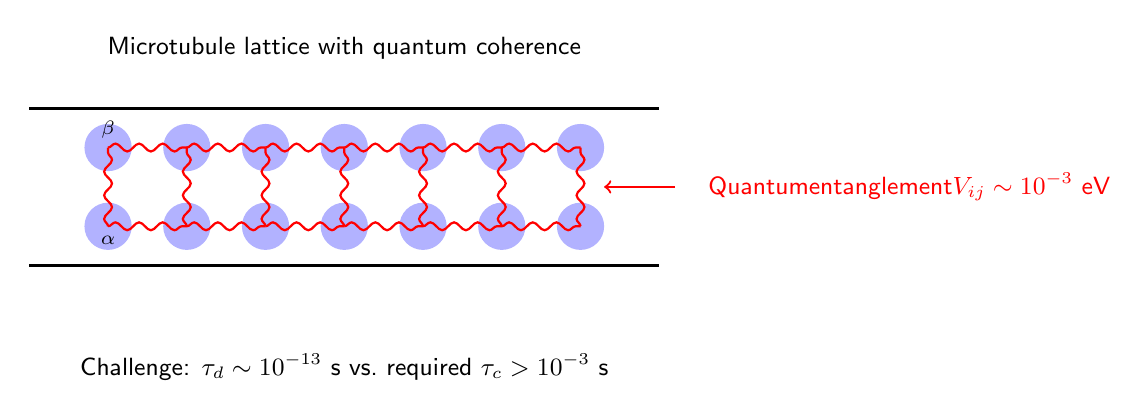
\begin{tikzpicture}[scale=1.0]
% Conceptual diagram of quantum coherence in microtubule
\draw[very thick] (-4,0) -- (4,0);
\draw[very thick] (-4,2) -- (4,2);

% Tubulin dimers as circles
\foreach \x in {-3,-2,-1,0,1,2,3} {
    \fill[blue!30] (\x,0.5) circle (0.3);
    \fill[blue!30] (\x,1.5) circle (0.3);
}

% Quantum coherence connections (wavy lines)
\foreach \x in {-3,-2,-1,0,1,2} {
    \draw[red,thick,decorate,decoration={snake,amplitude=0.5mm,segment length=3mm}] (\x,0.5) -- (\x+1,0.5);
    \draw[red,thick,decorate,decoration={snake,amplitude=0.5mm,segment length=3mm}] (\x,1.5) -- (\x+1,1.5);
}

% Vertical coupling
\foreach \x in {-3,-2,-1,0,1,2,3} {
    \draw[red,thick,decorate,decoration={snake,amplitude=0.5mm,segment length=3mm}] (\x,0.5) -- (\x,1.5);
}

% Labels
\node[above,font=\sffamily\small] at (0,2.5) {Microtubule lattice with quantum coherence};
\node[below,font=\sffamily\scriptsize] at (-3,0.5) {$\alpha$};
\node[above,font=\sffamily\scriptsize] at (-3,1.5) {$\beta$};

\node[right,font=\sffamily\small,red] at (4.5,1) {Quantum\\entanglement\\$V_{ij} \sim 10^{-3}$ eV};
\draw[red,thick,->] (4.2,1) -- (3.3,1);

% Decoherence representation
\node[below,font=\sffamily\small,align=center] at (0,-1) {Challenge: $\tau_d \sim 10^{-13}$ s vs.~required $\tau_c > 10^{-3}$ s};
\end{tikzpicture}
\end{center}

\textbf{Computational advantage:} Quantum parallelism $\rightarrow$ exponential speed-up for certain tasks (e.g., pattern recognition?)

\textbf{Problem:} No known biological algorithm requires quantum computation; classical neural networks already very powerful

\subsection{Vibronic Coherence at Room Temperature}

\textbf{Insight from VE-TFCC theory:} Strong vibronic coupling (electron-phonon interaction) can sustain thermal quantum coherence via Bogoliubov quasiparticles $\rightarrow$ stable coherent states at 310~K.

\textbf{Application to microtubules:} Aromatic residues (Trp, Tyr, Phe) have $\pi$-electron systems that couple to THz lattice vibrations $\rightarrow$ vibronic excitations.

\textbf{Coherence survival condition:}
\begin{equation}
g \omega \gtrsim k_B T
\end{equation}
where:
\begin{itemize}
\item $g$ = vibronic coupling constant
\item $\omega$ = phonon frequency (THz range)
\item $k_B T \approx 25$~meV at $T = 310$~K
\end{itemize}

For THz phonons at $\omega = 2\pi \times 1$~THz $= 4.1$~meV:
\begin{equation}
g_{\mathrm{required}} \gtrsim \frac{k_B T}{\omega} \approx 6
\end{equation}

\textbf{Testable prediction:} Measure quantum variance in microtubules:
\begin{equation}
\Delta q^2 = \langle q^2 \rangle - \langle q \rangle^2
\end{equation}
where excess variance (beyond classical thermal) indicates quantum coherence.

\textbf{Status:} Not yet measured experimentally

\section{Critical Challenges to Quantum Hypotheses}

\subsection{Decoherence Problem}

\textbf{Tegmark's calculation} (2000): Decoherence time in warm, wet brain environment:
\begin{equation}
\tau_d \sim \frac{\hbar}{E_{\mathrm{env}}} \sim 10^{-13}\ \mathrm{s}\ (100\ \mathrm{femtoseconds})
\end{equation}
where:
\begin{itemize}
\item $\tau_d$ = decoherence time
\item $E_{\mathrm{env}}$ = environmental interaction energy
\end{itemize}

\textbf{Dominant decoherence mechanisms:}
\begin{itemize}
\item Water dielectric fluctuations
\item Ion motion (Na$^+$, K$^+$, Ca$^{2+}$)
\item Thermal phonons ($k_B T \sim 25$~meV at 310~K)
\end{itemize}

\textbf{Decoherence rate estimate:}
\begin{equation}
\Gamma_{\mathrm{dec}} = \frac{1}{\tau_d} \sim 10^{13}\ \mathrm{s}^{-1}
\end{equation}

This is $10^{10}$ times faster than the required coherence time ($\tau_c > 1$~ms) for Orch-OR.

\textbf{Counter-arguments:}
\begin{itemize}
\item Tegmark assumed point dipoles; extended wavefunctions may decohere slower
\item Ordered water near microtubule surface reduces fluctuations
\item Vibronic coupling creates decoherence-free subspaces (VE-TFCC insight)
\end{itemize}

\textbf{Current status:} No consensus; experimental measurement needed

\subsection{Lack of Biological Function}

\textbf{Evolutionary argument:} If quantum effects were functionally important, we'd expect:
\begin{itemize}
\item Selection pressure to maintain coherence (e.g., specialized shielding proteins)
\item Deficits in organisms lacking microtubules (but prokaryotes have cognition without microtubules)
\end{itemize}

\textbf{Alternative explanation:} All known neural functions are explainable by classical electrophysiology.

\subsection{Anesthetic Paradox}

\textbf{Observation:} General anesthetics disrupt consciousness and bind to microtubules.

\textbf{Quantum interpretation:} Anesthetics disrupt THz coherence $\rightarrow$ loss of quantum computation $\rightarrow$ unconsciousness

\textbf{Classical interpretation:} Anesthetics alter microtubule-MAP interactions $\rightarrow$ disrupt synaptic vesicle transport $\rightarrow$ loss of neurotransmission

\textbf{Experimental test:} Does anesthetic binding shift THz resonances or reduce coherence times?
\begin{itemize}
\item \textbf{Preliminary data} (in vitro): Yes, small shifts ($\sim$0.1~THz)
\item \textbf{In vivo test}: Not yet done
\end{itemize}

\section{Worked Example: Microtubule Mechanical Analysis}

\textbf{Problem:} Calculate the force required to buckle a 10~$\mu$m microtubule segment under axial compression, and compare to typical cellular forces.

\subsection*{Given Parameters}

\begin{tabular}{@{}ll@{}}
Young's modulus & $E = 1.5$~GPa \\
Outer diameter & $D_{\mathrm{outer}} = 25$~nm \\
Inner diameter & $D_{\mathrm{inner}} = 15$~nm \\
Segment length & $L = 10$~$\mu$m \\
\end{tabular}

\subsection*{Step 1: Calculate Second Moment of Area}

For a hollow cylinder:
\begin{equation}
I = \frac{\pi}{64}(D_{\mathrm{outer}}^4 - D_{\mathrm{inner}}^4)
\end{equation}
\begin{equation}
I = \frac{\pi}{64}[(25 \times 10^{-9})^4 - (15 \times 10^{-9})^4] = 1.53 \times 10^{-32}\ \mathrm{m}^4
\end{equation}

\subsection*{Step 2: Calculate Buckling Force}

Using Euler's formula for a pinned-pinned column:
\begin{equation}
F_{\mathrm{buckle}} = \frac{\pi^2 EI}{L^2}
\end{equation}
\begin{equation}
F_{\mathrm{buckle}} = \frac{\pi^2 \times (1.5 \times 10^9) \times (1.53 \times 10^{-32})}{(10 \times 10^{-6})^2} = 2.26 \times 10^{-12}\ \mathrm{N} = 2.26\ \mathrm{pN}
\end{equation}

\subsection*{Step 3: Compare to Cellular Forces}

\begin{center}
\begin{tabular}{@{}lrl@{}}
\toprule
Force Source & \multicolumn{1}{c}{Force (pN)} & Comparison \\
\midrule
Kinesin motor & 5--7 & \textbf{Exceeds buckling force} \\
Dynein motor & 5--7 & \textbf{Exceeds buckling force} \\
Chromosome segregation & 10 & \textbf{4$\times$ buckling force} \\
Microtubule buckling & \textbf{2.3} & Baseline \\
\bottomrule
\end{tabular}
\end{center}

\subsection*{Conclusion}

The calculated buckling force ($\sim$2.3~pN) is \textbf{lower than typical cellular forces} (5--10~pN), meaning microtubules can buckle under compression from motor proteins or mitotic forces. This necessitates:
\begin{itemize}
\item Stabilization by MAPs (tau, MAP2) to increase effective stiffness
\item Crosslinking to adjacent microtubules to prevent buckling
\item Dynamic turnover to remove buckled microtubules
\end{itemize}

\section{Applications}

\subsection{Neurodegeneration Research}

\textbf{Tau pathology in Alzheimer's disease:}
\begin{itemize}
\item Hyperphosphorylated tau detaches from microtubules
\item Microtubules destabilize $\rightarrow$ impaired axonal transport
\item Cargo accumulation contributes to neuronal death
\item \textbf{Therapeutic strategy:} Microtubule stabilizers (e.g., epothilone D) in clinical trials
\end{itemize}

\subsection{Cancer Chemotherapy}

\textbf{Microtubule-targeting agents:}
\begin{itemize}
\item \textbf{Taxanes (paclitaxel, docetaxel)}: Stabilize microtubules $\rightarrow$ block mitosis $\rightarrow$ apoptosis
\item \textbf{Vinca alkaloids (vincristine, vinblastine)}: Destabilize microtubules $\rightarrow$ mitotic arrest
\item \textbf{Mechanism:} Rapidly dividing cancer cells most sensitive to mitotic disruption
\item \textbf{Clinical use:} Breast, ovarian, lung, and hematological cancers
\end{itemize}

\subsection{Quantum Biology Experimental Platform}

\textbf{Microtubules as test systems for room-temperature quantum effects:}
\begin{itemize}
\item Well-characterized structure (25~nm, 13 protofilaments)
\item Accessible to THz spectroscopy
\item Testable with 2D THz, pump-probe, and NV-diamond magnetometry
\item \textbf{If quantum effects confirmed:} Implications for consciousness theories and quantum computing substrates
\end{itemize}

\subsection{Synthetic Biological Materials}

\textbf{Biomimetic applications:}
\begin{itemize}
\item Self-assembling nanotubes for drug delivery
\item Dynamic scaffolds for tissue engineering
\item Bio-inspired actuators using motor proteins on microtubule tracks
\item Molecular computing substrates (classical or quantum)
\end{itemize}

\section{Summary}

\begin{center}
\begin{tabular}{@{}p{4cm}p{5cm}p{5cm}@{}}
\toprule
\textbf{Aspect} & \textbf{Established Science} & \textbf{Speculative Quantum Theory} \\
\midrule
\textbf{Structure} & 25~nm hollow cylinder, 13 protofilaments, $\alpha$-$\beta$ tubulin dimers & Same \\
\midrule
\textbf{Function} & Structural support, transport tracks, mitotic spindle, cilia/flagella & Proposed: quantum computation substrate \\
\midrule
\textbf{Dynamics} & Dynamic instability ($v_+ \sim 2$ $\mu$m/min, $f_{\mathrm{cat}} \sim 0.01$ s$^{-1}$) & Proposed: coherence modulation \\
\midrule
\textbf{Coherence time} & N/A (classical) & Required: $\tau_c > 1$~ms; Calculated: $\tau_d \sim 10^{-13}$~s \\
\midrule
\textbf{Evidence} & Extensive structural, biochemical, cell biological & None experimental; theoretical models only \\
\midrule
\textbf{Medical relevance} & Alzheimer's (tau), cancer drugs (taxanes, vinca alkaloids) & Proposed: anesthetic mechanism \\
\midrule
\textbf{Status} & Well-established (Nobel Prize 2022 for GTPase mechanisms) & Highly speculative; requires experimental test \\
\bottomrule
\end{tabular}
\end{center}

\begin{keyconcept}
\textbf{Key Takeaway:} Microtubules are essential cytoskeletal structures with well-understood classical functions. The hypothesis that they enable quantum information processing in neurons remains unproven and faces severe challenges from decoherence. Experimental tests (THz spectroscopy, coherence measurements) are needed to resolve this controversy.
\end{keyconcept}

\section{Further Reading}

\textbf{Within this book:}
\begin{itemize}
\item \textbf{Orchestrated Objective Reduction (Orch-OR):} Detailed treatment of Penrose-Hameroff consciousness theory
\item \textbf{Quantum Coherence in Biological Systems:} General framework for warm quantum effects
\item \textbf{THz Resonances in Microtubules:} Vibrational modes proposed to sustain coherence
\item \textbf{Terahertz Technology:} Experimental probes for testing quantum hypotheses
\end{itemize}

\textbf{Key references:}

\textit{Structure and Function (Established):}
\begin{enumerate}
\item \textbf{Nogales et al., \emph{Nature} 391, 199 (1998)} --- Tubulin crystal structure (foundational)
\item \textbf{Mitchison \& Kirschner, \emph{Nature} 312, 237 (1984)} --- Dynamic instability discovery
\item \textbf{Desai \& Mitchison, \emph{Annu. Rev.~Cell Dev. Biol.} 13, 83 (1997)} --- Microtubule dynamics review
\end{enumerate}

\textit{Quantum Hypotheses (Speculative):}
\begin{enumerate}
\setcounter{enumi}{3}
\item \textbf{Penrose \& Hameroff, \emph{Phys. Life Rev.} 11, 39 (2014)} --- Orch-OR consciousness theory
\item \textbf{Hameroff \& Penrose, \emph{J. Conscious. Stud.} 21, 126 (2014)} --- Orch-OR update
\end{enumerate}

\textit{Critical Perspectives:}
\begin{enumerate}
\setcounter{enumi}{5}
\item \textbf{Tegmark, \emph{Phys. Rev.~E} 61, 4194 (2000)} --- Decoherence calculation (skeptical)
\item \textbf{Koch \& Hepp, \emph{Nature} 440, 611 (2006)} --- Critique of quantum consciousness
\end{enumerate}

\textit{Vibronic Coupling:}
\begin{enumerate}
\setcounter{enumi}{7}
\item \textbf{Bao et al., \emph{J. Chem. Theory Comput.} 20, 4377 (2024)} --- VE-TFCC theory (thermal coherence)
\end{enumerate}
